% 中点四边形 引入：任意四边形 ABCD 四边中点 E,F,G,H 连成 EFGH（含对角线）
\documentclass[tikz,border=4pt]{standalone}
\usepackage{ctex}
\usepackage{amsmath}
\usetikzlibrary{calc, decorations.markings}
\begin{document}
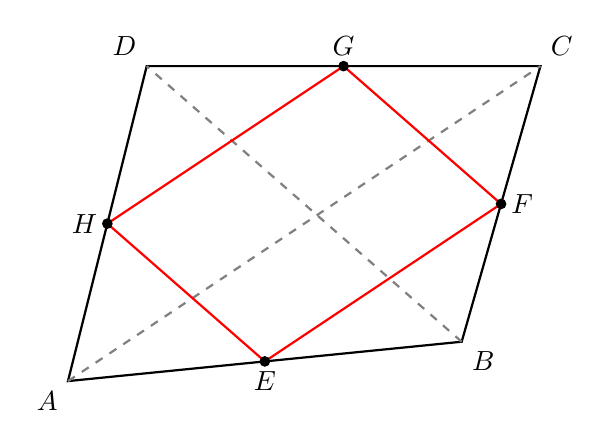
\begin{tikzpicture}[scale=1.0, thick]
  \coordinate (A) at (0,0);
  \coordinate (B) at (5,0.5);
  \coordinate (C) at (6,4);
  \coordinate (D) at (1,4);
  \coordinate (E) at ($(A)!0.5!(B)$);
  \coordinate (F) at ($(B)!0.5!(C)$);
  \coordinate (G) at ($(C)!0.5!(D)$);
  \coordinate (H) at ($(D)!0.5!(A)$);
  \draw (A)--(B)--(C)--(D)--cycle;
  \draw[gray, dashed] (A)--(C);
  \draw[gray, dashed] (B)--(D);
  \draw[red] (E)--(F)--(G)--(H)--cycle;
  \foreach \pt in {E,F,G,H} \filldraw (\pt) circle (1.5pt);
  \node[below left] at (A) {$A$};
  \node[below right] at (B) {$B$};
  \node[above right] at (C) {$C$};
  \node[above left] at (D) {$D$};
  \node[below] at (E) {$E$};
  \node[right] at (F) {$F$};
  \node[above] at (G) {$G$};
  \node[left] at (H) {$H$};
\end{tikzpicture}
\end{document}
